\chapter{Simulation der Ionenoptik}
\label{chap:Simulation}
Eine Simulation der Ionenoptik des Massenspektrometers ist sinvoll, um die Messergebnisse zu überprüfen, die Genauigkeit des Massenspektrometers zu bestimmen und Optimierungsansätze herrauszuarbeiten. Dafür wird das Programm \textit{SIMION} genutzt, das die Bewegung von geladenen Teilchen in elektrischen und magnetischen Feldern simulieren kann. Im Vergleich zu anderen Programmen ist \textit{SIMION} besonders geeignet, da es auf Ionen- und Elektronenoptik spezialisiert ist und die Möglichkeit bietet, die Simulationen mit geringem Aufwand mit eigenen Programmen zu erweitern. Im Folgenden soll die Methodik der Simulation und die Limitationen erläutert werden und im Anschluss die Ergebnisse der Simulationen präsentiert werden.

\section{\textit{SIMION}: Methodik und Limitation}
Zu Grunde der Simulationen liegt bei \textit{SIMION} die numerische Lösung der Laplace-Gleichung (\ref{eq:laplace}) für das elektrische Potential $\Phi$ in einem gegebenen Raum \cite{SIMION}.
\begin{equation}
    \label{eq:laplace}
    \nabla^2 \Phi = 0.
\end{equation}
Um diese partielle Differentialgleichung zu lösen, nutzt das Programm finite Differenzverfahren (FDM), mit denen eine Ableitung über die Differenz zweier benachbarter Punkte approximiert wird. Dafür muss der Raum diskretisiert, also in ein Gitter aus Punkten aufgeteilt werden. Dabei ist es möglich mehrere Gitter mit verschiedenen Auflösungen zu definieren und diese innerhalb einer Simulation zu nutzen. Damit die iterative Lösung der Laplace-Gleichung schnell konvergiert, wird Überrelaxation (engl. \textit{Optimized Over-Relaxation, OOR}) verwendet. Statt bei jeder Iteration exakt nach der FDM zu aktualisieren, wird eine gewichtete Mischung aus der neuen und alten Lösung genommen. Um das Potential eines Gitters in jedem Punkt errechnen zu können, werden als Randbedingungen vom Nutzer definierte Elektroden und die Ränder der Simulation verwendet.
Elektroden bilden dabei Dirichlet-Randbedinungen, welche das genaue Potential an dem Ort festlegen. Für die Ränder der Simulation werden Neumann-Randbedinungen angenommen, die die Ableitung des Potentials entlang der zum Rand normalen Richtung festlegen. Diese werden auf 0 definiert, was den Vorteil hat, dass sich das Elektrische Feld 
\begin{equation}
    \vec E = -\nabla \Phi
\end{equation}
außerhalb des Simulationsbereiches so fort setzt, als ob er sich in einem unendlichen Raum befindet \cite{SIMION}.

Das elektrische Feld $E$ kann dann mit dem errechneten Potential an jedem Ort bestimmt werden, um die Beschleunigung der Lorentzkraft auf geladene Teilchen zu ermitteln. Für die Iteration der Trajektorien wird eine Runge-Kutta-Verfahren 4. Ordnung angewandt. Die zeitliche Schrittweite ist dabei variabel. In einer Simulation werden vom Nutzer definierte Teilchen nach einander in das Feld gesetzt und ihre Trajektorie berechnet. 

Limitierend ist allgemein, dass die Teilchen dabei selbst nicht das Potential beeinflussen. Das bedeutet, dass sie auch nicht miteinander wechselwirken können und keine Raumladungseffekte berücksichtigt werden. Da innheralb dieser Arbeit aber unter Einzelstoßbedinungen gearbeitet wird, ist das nicht relevant. Angenommen wird auch, dass die Felder statisch sind und somit werden zeitabhängige Effekte, wie dem Induktionsgesetz, nicht berücksichtigt. Es ist aber trotzdem möglich die Felder in Abhängigkeit der Zeit mit eigener Programmierung zu verändern. Solange die Frequenz der Änderung nicht zu hoch ist, können sie weiterhin als quasi-statisch angenommen werden.

\section{Modellierung und Konfiguration}
Um die Ionenoptik der derzeit verwendeten Geometrie zu untersuchen, muss dieser akkurat modelliert werden. Anhand der originalen Designdateien des Plattenkondensators konnte eine vereinfachte Geometrie in \textit{SIMION} erstellt werden. Die Elektroden wurden zweidimensional modelliert und dann mit Zylindersymmetrie auf 3D erweitert. Abbildung \ref{fig:model} zeigt das Modell des Massenspektrometers in \textit{SIMION}. Zunächst wurden die derzeitigen Maße der Anlage eingesetzt, anhand der Simulation soll aber der Abstand des Detektors variiert werden.

\begin{figure}
    \centering
    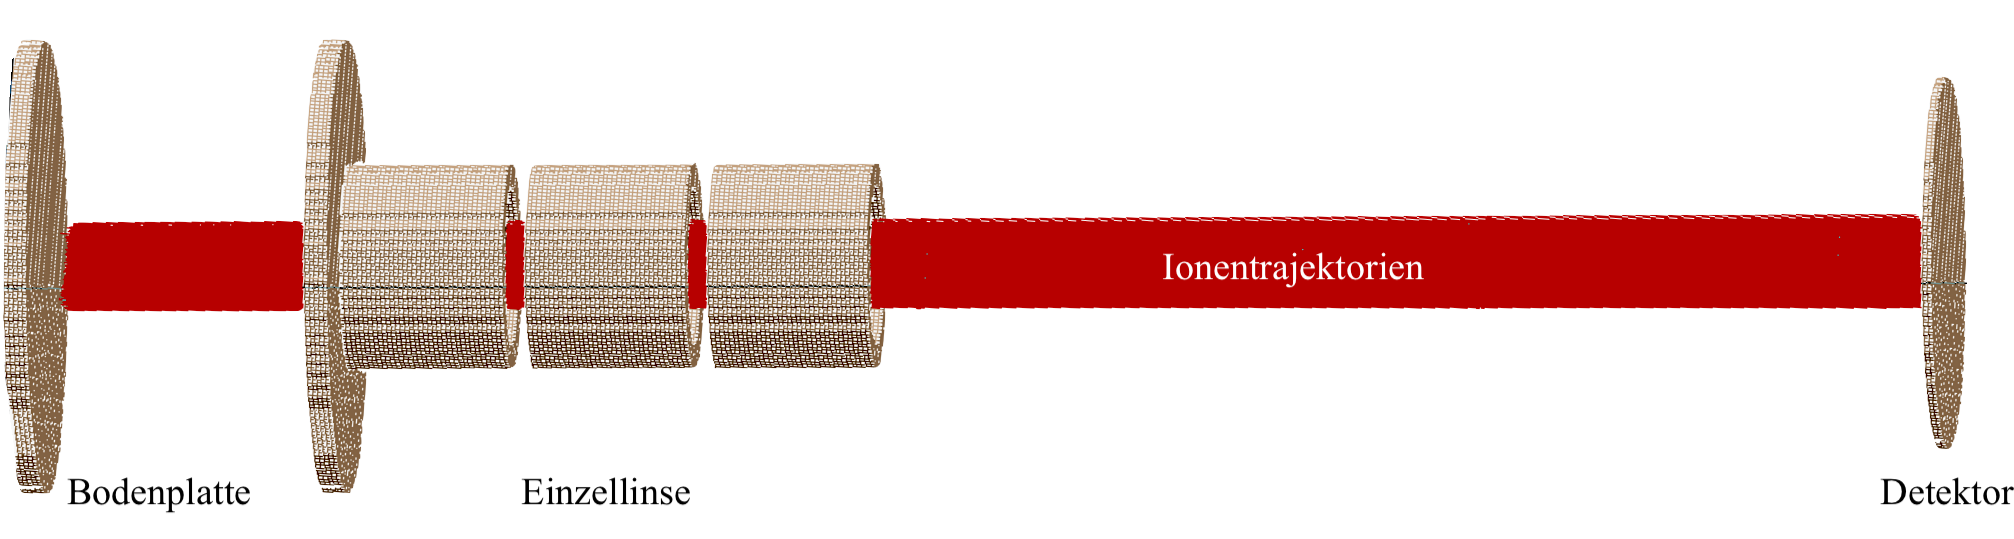
\includegraphics[width=1\textwidth]{Model.png}
    \caption[Modell des Massenspektrometers in \textit{SIMION}]{Modell des Massenspektrometers in \textit{SIMION}. Die Elektroden sind in beige dargestellt, die Flugbahnen der Ionen in rot.}
    \label{fig:model}
\end{figure}

Auf der Bodenplatte (in der Simulation links) wird ein positives Potential von mehreren Kilovolt angelegt, während die Deckenplatte und Einzellinse auf Masse (0 V) liegt. Genauso wie im Experiment wird die Linse vorerst nicht verwendet. Der Detektor (in der Simulation rechts) bekommt ein Potential von -2500 V, ähnlich dem in der Anlage. 

Die Interaktion der Elektronen mit dem Neutralgas wird in der Simulation nicht berücksichtigt. Stattdessen werden die Ionen im Pfad des Elektronenstrahls erschaffen, also in einer Linie paralell zu den Platten. Um die räumliche Ausdehnung des Strahls zu berücksichtigen und, wie auch im Experiment zu beobachten, eine Verteilung der Flugstrecken der Ionen zu erhalten, wird das in der Auswertung des Strahlprofils bestimmte Profil des Strahls genutzt. Die Ionen werden dann mit einer FWHM von $1.95$ mm um die Linie des Strahls gauß-verteilt. Da das Experiment von der Einzelstoßbedingung ausgeht, kann ein Ion nach dem Anderen simuliert werden und die Wechselwirkung zwischen Ionen vernachlässigt werden.

Die Art der Teilchen, so wie ihre Häufigkeitsverteilung können mit einem \textit{.fly2}-File definiert werden. Auch die räumliche Verteilung des Strahls wurde hierüber implementiert. Die verwendete Datei ist im Anhang \ref{fly2} zu finden. Für die kinetische Energie der Teilchen wird 1/25 eV angenommen. Dieser Wert ergibt sich, wenn man eine Maxwell-Boltzmann-Verteilung für die kinetische Energie der Ionen annimmt und die Temperatur der Ionen auf 300 K (Raumtemperatur) setzt: 
\begin{equation}
    \label{eq:kin}
    \left< E_{\text{kin}} \right> = \frac{3}{2} k_B T_{Raum} \approx \frac{1}{25} \text{ eV}.
\end{equation}

Um dieselben Informationen aus der Simulation zu gewinnen, wie sie auch im Experiment vom Detektor aufgenommen werden, werden Flugzeit und Position jedes Teilchens zum Auftreffpunkt aufgezeichnet. Diese können dann mit den selben Methoden wie die experimentellen Daten ausgewertet werden. Im Folgenden werden verschiedene Simulationen durchgeführt, um die Ionenoptik zu untersuchen. Dafür sollen zunächst die Ergebnisse aus dem Experiment nachsimuliert werden, um die Genauigkeit der Simulation zu überprüfen. 
